\chapter{Introduction}\label{ch:intro}

In this chapter we are going to describe accurately the problem and provide a possible 
solution (from the point of view of a Distributed Systems designer).\\


\section{The Problem}

The bridge has a \textbf{maximum capacity} $c \geq 1$ and a crossing time $t$. \\

%TODO se passa un blocco di macchine c ci mette c turni o un turno solo?\\
%TODO il processo ambiente quindi mette in comunicazione una macchina 
%sia con la macchina dietro che con quella davanti?\\ 
%TODO se turni o a secondi\\

Cars can send messages to adjacent cars (to the car in front and to the rear one); 
cars can also have the ability to speak with more than two other cars depending on the 
\textbf{power of their transmission medium} $p \geq 1$.\\

The initialization of a communication between two cars can be done unsing an 
\textbf{environment process} 
that returns the required references needed to start the message exchange.\\

So basically a car can only send messages to the $p$ cars in front and 
to the $p$ cars behind. We assume that the bridge length doesn't constitute an impediment 
for the communications (so even if the bridge was very long, however, 
the cars can send messages as if they were close).\\

For simplicity we assume that every car has the 
same dimensions expressed in an arbitrary length scale called \textbf{block} and 
\textbf{every measure is an integer} ($s$, $l$, $c$, $p$, etc.). \\

We assume that cars can have a failure at any moment and there are only 
three types of failures:
\begin{itemize}
    \item \textbf{engine failure} (the car cannot move but can send help messages to the other cars)
    \item \textbf{link failure} (the car can move but cannot send any message)
    \item \textbf{system failure} (the car cannot move and cannot send messages)
\end{itemize}

We assume that a link failure is equivalent to a system failure cause the car cannot 
take any decision without the agreement of the others. 
In case of engine failure or system failure the car or another helping car must call 
a tow truck in order to remove the broken car 
(in this case we have to wait an \textbf{elimination time} $e$).
In case of failure the car behind has to wait until the tow truck removes the broken car.\\

We assume that a car cannot be malicius (must follow the algorithm) but the communication 
channel isn't secure so it is exposed to a \textbf{MIM} (man in the middle) attack 
(drop messages, edit messages, message injection, ...).\\

Finally we have to consider that in a distributed system a global up-to-date state 
or a global timing cannot exist; this implies that each car can have a partial 
and \textbf{inconsistent view} of the global environment and a \textbf{time drift} 
from the global time (for this reason the system cannot guarantee the FIFO ordering 
at all).

\begin{figure}[h]
    \centering
    \resizebox{12cm}{5cm}{%
    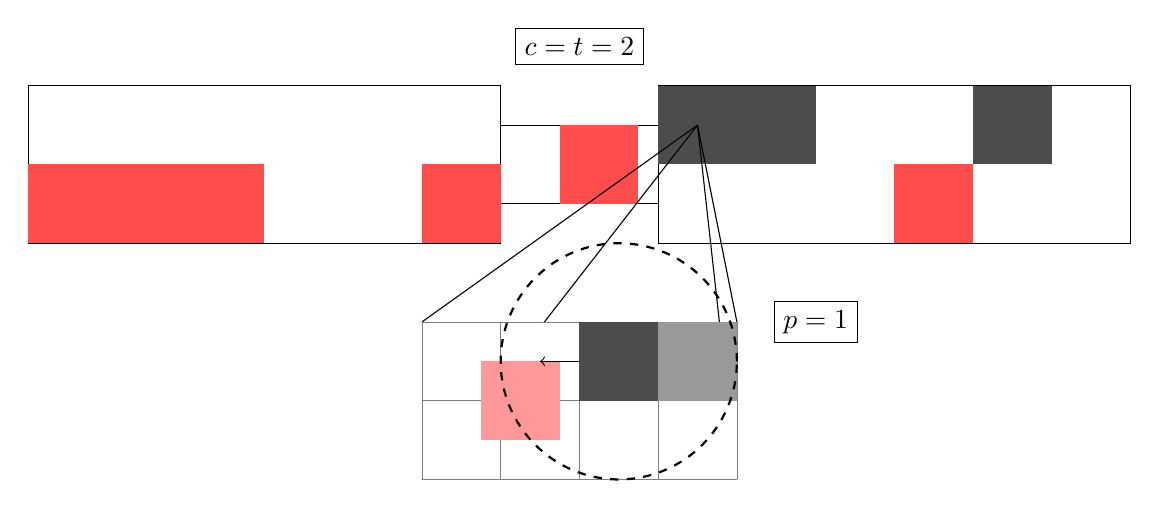
\begin{tikzpicture}
        % queues
        \draw (1,-1) rectangle (7,1);
        \draw (-7,-1) rectangle (-1,1);
        
        % bridge
        \draw (-1,-0.5) rectangle (1,0.5);
        \fill[red!70!white] (-0.25,-0.5) rectangle (0.75,0.5);
        \fill[red!70!white] (4,-1) rectangle (5,0);
        \node[draw,align=left] at (0,1.5) {$c = t = 2 $};
        
        % left cars
        \fill[red!70!white] (-7,-1) rectangle (-6,0);
        \fill[red!70!white] (-6,-1) rectangle (-5,0);
        \fill[red!70!white] (-5,-1) rectangle (-4,0);
        \fill[red!70!white] (-2,-1) rectangle (-1,0);
        
        %% right cars
        \fill[black!70!white] (1,0) rectangle (2,1);
        \fill[black!70!white] (2,0) rectangle (3,1);
        \fill[black!70!white] (5,0) rectangle (6,1);
        
        \draw[black] (1.5,0.5) -- (-2, -2);
        \draw[black] (1.5,0.5) -- (2, -2);
        \draw[black] (1.5,0.5) -- (-2, -4);
        \draw[black] (1.5,0.5) -- (2, -4);

        % grid
        \fill[white]  (-2,-4) rectangle (2, -2);
        \draw[step=1cm,gray,very thin] (-2,-4) grid (2, -2);
        \fill[black!70!white] (0,-3) rectangle (1,-2);
        \fill[black!40!white] (1,-3) rectangle (2,-2);
        \fill[red!40!white] (-1.25,-3.5) rectangle (-0.25,-2.5);

        \draw[black,thick,dashed] (0.5,-2.5) circle (1.5cm);
        \node[draw,align=left] at (3,-2) {$p = 1$};
        \draw[->,black] (0,-2.5) -- (-0.5, -2.5);
    \end{tikzpicture}
    }
    \caption{Example of a possible situation} \label{fig:1}
\end{figure}


\section{Subproblems}

Following the \textit{divide et impera} philosophy now we are going to split the problem 
into some subproblems and solve them. 


\subsection{Starvation/deadlock and order method}

Ideally a car that reaches first the queue must pass before other 
incoming cars (\textbf{FIFO}).\\

We have to \textbf{avoid starvation} (ie. when a car waits infinite time cause the opposite queue 
has infinite lenght and it never has the priority) and \textbf{deadlock} (cars aren't able to 
reach the agreement). 


\subsection{Solution}

In order to avoid \textbf{starvation} in a first stage cars syncronize themselves 
(for the syncronization process we follow the \textbf{Berkeley algorithm})
in terms of local timinig and in a second stage there will be a \textbf{leader election} 
and the leader decides the crossing order. Using this method we also avoid 
the possibility of a \textbf{deadlock} as long as the leader is running.\\

In a certain instant the elected leader is the first car that has reached the bridge; 
once the current leader cross the bridge there is a new election of the car on the other 
side of the bridge (if one is present).\\


\section{Syncronization problem}

Every car has a \textbf{local timing} that can \textbf{drifts} out from the 
global timing. 

\subsection{Solution}

So we need to syncronize the incoming cars using the \textbf{Berkeley algorithm}.\\

A new incoming car calls the \textit{environment:get$\_$adjacent$\_$cars(p)} 
method in order to get the name of the adjacent cars. \\

The new car $c$ sends a message to the nearest car $n$ in order to get the current time 
(we assume that $n$ was already syncronized). 
With this information $c$ is concious of the RTT and its local drift from the global time. 
Finally $c$ sends to the furthest car 
reachable in the queue its arrival time (and the message is propagated along the 
peer chain to the current leader).\\

So basically the global timing is the timing of the first leader (or the average time 
of the first block of incoming cars).\\

If some new unsyncronized cars appear in block the syncronization process takes into 
consideration the average RTT (according to the Berkeley algorithm). 


\section{Agreement}

The current leader identifies the block of cars that will cross the bridge and notifies
this decision.  

\subsection{Solution}

The leader is concious of the current queue state in terms of arrival time of the cars; 
so it decides how may cars have to cross the bridge in this turn (accordingly with the 
bridge capacity c and FIFO ordering).\\

Finally the leader notifies to the involved cars its decision and, after 
an acknowledgement (agreement), the block starts crossing. 


\section{Failures}

In case of failure another car (or the same car) has to call a \textbf{tow truck} for help.


\subsection{Solution}

Each car recursively checks if other reachable cars are safe; if a check message
hasn't any response before a certain \textbf{timeout} (depends on the RTT) is assumed 
that the receiver has a failure (and so the tow truck will be call).


\section{MIM attack}

The system must withstand a MIM attack.


\subsection{Solution}

Each message will be encrypted (HTTPS).


\section{Scalability}

The system must \textbf{scale wrt. the load} 
(the number of cars and clients can scale arbitrary).


\subsection{Solution}

Assume that the available machines are defined in an arbitrary 
way in the initialization phase; on each machine some docker containers 
will be raised and foreach one of those an arbitrary number of web services and 
car processes will be spawned.\\

We will design an embedded load balancer in order to avoid the web services overload 
(considering the number of calls).


\section{SPOF}

The system must be resilient wrt. failures (even multiple failures);
so basically the architecture must be deeply \textbf{distributed} 
and \textbf{decentralized} (avoid any SPOF). 


\subsection{Solution}

The scalability requirement imposes that every macro-component must be scalable 
so the architecture provides some \textbf{peer-to-peer layers} 
(web services layer, cars layer).
The only SPOF in this context can be the \textit{environment} component 
(which is embedded into the web services) that allows for a new spawned car to 
start a message exchange with the adjacent cars. 
A possible solution can be using a \textbf{distributed DBMS} like Mnesia~\cite{1} in order to keep 
track of the queue state.